\Chapter{Koncepció}

\Section{Hasonló rendszerek, megoldások áttekintése}

Az Amazonnak már működő szállítási rendszere van, mely drónnal 30 percen belül eljuttatja a 2,3 kg-nál kisebb tömegű csomagokat az ügyfelekhez.
Ezek a drónok csak 24 km-es hatótávval rendelkeznek, így csak akkor biztonságos egy kézbesítés ha a célállomás maximum 12 km-re van.
A csomag maximum térfogatáról nincsenek pontos adatok.
Ezt a rendszert \textit{Prime Air}-nek hívják \cite{prime-air}. Az Amazon Prime Air egy drónja látható \aref{fig:prime}. ábrán.

\begin{figure}[h]
    \centering
    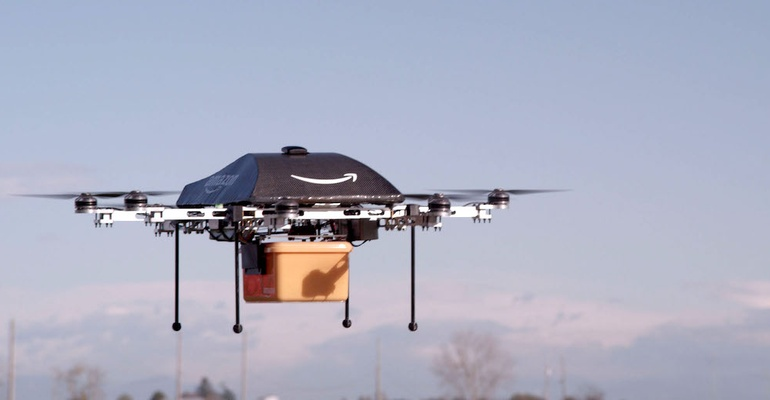
\includegraphics[scale=0.4]{images/prime.jpg}
    \caption{Amazon Prime Air drón}
    \label{fig:prime}
\end{figure}

Először 2016-ban próbálták ki, azóta még nem sikerült bevezetni különböző jogi korlátozások miatt. Olyan jogi elvárásoknak kell megfelelni, mint például az alábbiak.
\begin{itemize}
    \item Muszáj egy drón pilótának ellenőrizni a repülést és szükség esetén kötelező közbeavatkoznia.
    \item Egy ilyen pilóta csak 1 drónt felügyelhet egyszerre, kivéve ha rendelkezik több felügyeletéhez megfelelő engedéllyel.
    \item A drónokat nem lehet közvetlen egy személy vagy gépjármű fellett működtetni.
    \item Problémát jelent továbba, hogy nem minden légtér megfelelő a drónokkal való szállításra. A reptér mellett fekvő nagyvárosokban például biztos hogy nem lehet drónokkal szállítani.
    \item A csomagot szállító drónnak is kell rendelkeznie engedéllyel, hogy alkalmas kereskedelmi szállításra.
\end{itemize}

Az FAA 2020-ban engedélyezte az Amazonnak a drónokkal való csomagszállítást, de egyelőre csak tesztelik a technológiát pár városban.A jövőben teljesen elképzelhető, hogy a csomagok felét drónok szállítják ki. Önmagában az Amazon naponta átlagosan 7 millió csomagot szállít ki, és bevallásuk szerint a csomagok 86\%-a drónnal szállítható lenne.

Az Amazon felhőszolgáltásai között is található olyan szolgáltatás, amellyel könnyedén kezelhetjük az IoT eszközöket, jelen esetben a drónokat.
Ilyen az \textit{IoT Core} vagy az \textit{IoT Things Graph} amin grafikus felületen összeköthetjük és beállíthatjuk az eszközeink közötti kommunikációt.
A DHL is próbálkozott hasonló csomagkézbesítő megoldásokkal. Ők egy úgynevezett  \textit{Parcelcopter}-el szállították a csomagokat (\ref{fig:parcelcopter}. ábra).

\begin{figure}[h]
    \centering
    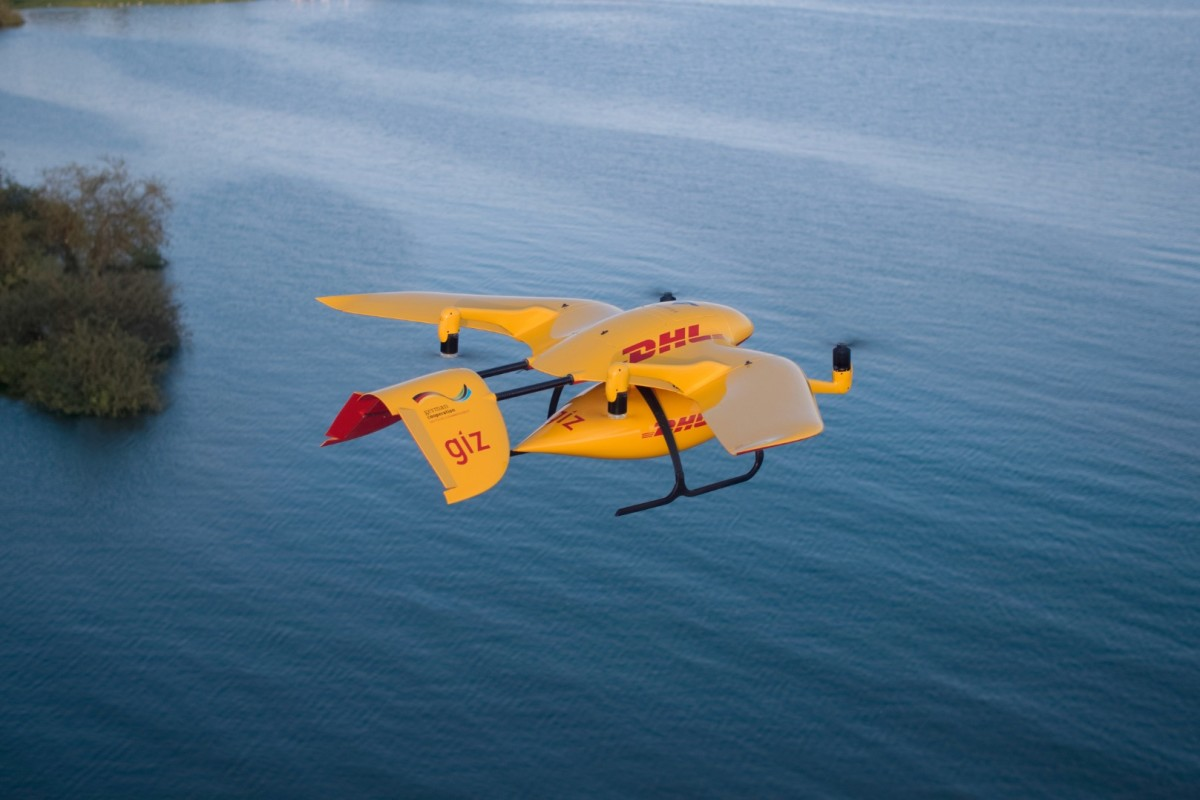
\includegraphics[scale=1.0]{images/parcelcopter.jpeg}
    \caption{DHL Parcelcopter V4.0}
    \label{fig:parcelcopter}
\end{figure}

A DHL Percelcopter alapvetően más problémát akar megoldani, a nagyon nehezen elérhető helyekre probálnak csomagokat szállítani.

A \textit{FlytBase} \cite{flyt} vállalat már kínál szoftveres megoldásokat drónok automatizációjára és valós idejű figyelésére és irányítására, útvonal tervezésre valamint flotta menedzselésre.
Már van kész megoldásuk a következőkre:
\begin{itemize}
    \item Biztonsági megfigyelések
    \item Automatikus dokkolás állomásokhoz
    \item Veszélyhelyzetre reagálás, ez lehet vér, szerv vagy gyógyszer szállítás.
    \item Csomag szállítás
\end{itemize}

Elterjedt termékük a FlytNow, ami úgy működik, hogy a drónunkat összekötjük egy appon keresztül a felhőben lévő FlytNow rendszerrel,
majd internetet keresztül elérünk egy verzérélőpultot \ref{fig:flytdash} amin irányíthatjuk a drónjainkat és láthatjhuk az adatokat.
Ez a rendszer arra összpontosít hogy gyorsan, bonyolult telepítés és beállítás nélkül tudjunk drónokat irányítani.
Ezt a rendszer magánembereknek és cégeknek egyaránt elérhető, több csomagban.
Van egy másik FlytWare nevű termékük raktár menedzselésre és logisztikai feladatokra. Olyan feladatokra specializálódnak a drónok mint a bárkód szkennelés,
zárt környezetben repülés. Természetesen a raktár adatait elérjük a rendszer vezérlőpultján. Így például egy leltár sokkal egyszerűbben megoldható.


\begin{figure}[h]
    \centering
    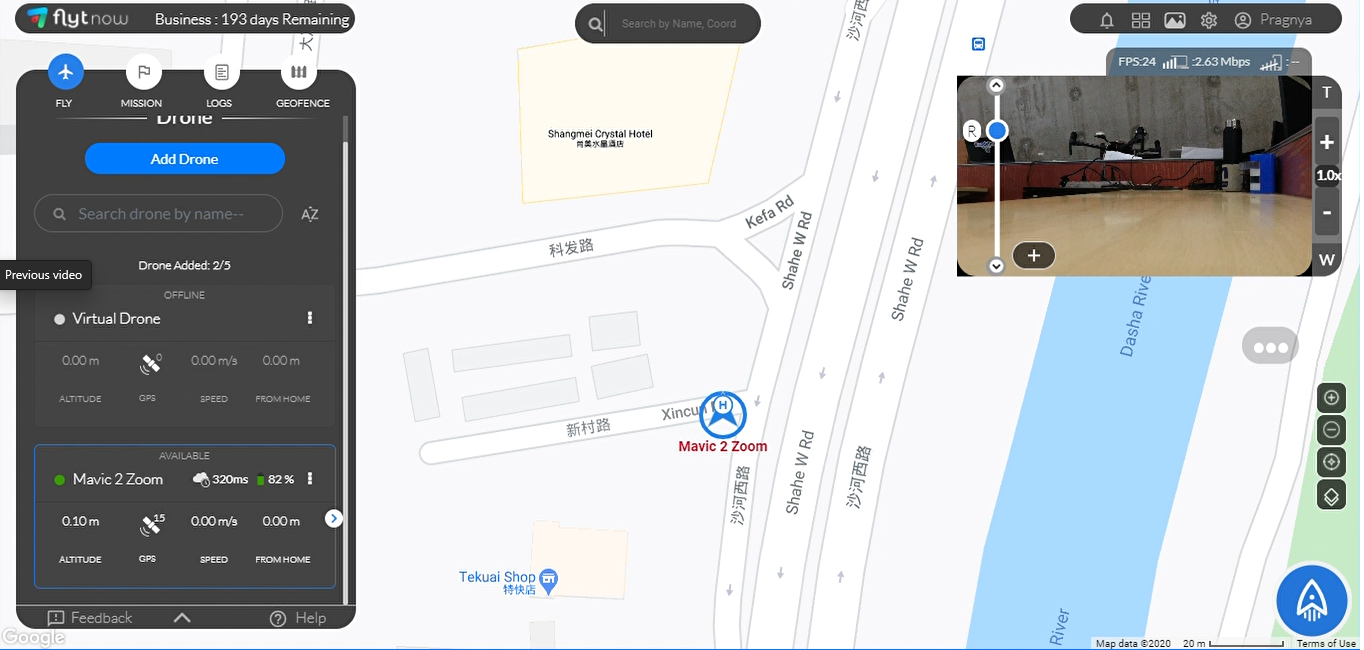
\includegraphics[scale=0.3]{images/flyt-dashboard.png}
    \caption{Flytnow livestream dashboard}
    \label{fig:flytdash}
\end{figure}

Az \textit{ANRA Techonlogies}\cite{anra} cég is foglalkozik mindenféle drón irányítás, megfigyeléssel. A SmartSkies néven futó rendszere például drónokat használ mindenféle szenzorral,
ahhoz hogy a pontosabb adatokat kapjunk megfigyeléses mérésekhez. Például egy olyan légtérben ahol rengeteg drón repül előfordulhatnak hibák, egy drón rossz adatokat küld helyzetéről vagy
teljesen megszűnik a kommunikáció, esetleg idegen tárgyak akadályozzák a légtérben  való forgalmat, stb.
Ebben a rendszerben minden drón el van látva radarral, kamerával és más szenzorokkal. Így az összegyűjtött adatokat kombinálva
egy sokkal pontosabb képet kapunk ami hasznos a navigációhoz, és akár fél percre előre meg tudjuk mondani mi lesz az adatok alapján, előre jelezve az esetleges hibákat.


A \textit{BeeCluster}\cite{beecluster} egy nyílt forráskódú, Golang-ban írt drón orchesztrációs rendszer. Előnye, hogy prediktív optimizációt használ.
Tehát a feladatok előtt egy eszimulációt futtat, ami alapján optimalizálja, azaz hatékonyabbá és gyorsabbá teszi a valós folyamatot.
Olyan feladaotkra használják mint a földrajzi térképezés, wifi lefedettség térkép, új utak feltérképezése.



\Section{A szállítási probléma absztrakt modellje}

A szállítási modellünk alapvetően úgy nézne ki, hogy a raktár és a kiszállítási hely közti távolság függvényében a csomagokat a raktárból drónok, vagy drónokkal felszerelt teherautók viszik ki.
A teherautók a kiszállítási hely közelében használnák a drónokat hogy kézbesítsék a csomagokat.

Feltételezzük, hogy a drón és a csomag ugyanazon a raktárba vagy tehergépkocsiba található, de a szimuláció szemszögéből nem fontos hogy raktár vagy tehergépkocsi, az a lényeges, hogy egy helyen található, és a drón automatikusan fel tudja venni az adott csomagot
valamilyen rendszeren keresztül, kevesebb mint 5 perc alatt.

A drónok 3G, 4G vagy 5G hálózaton kommunikálnának az adatközpontokkal.
Az adott hálózaton elérhető sávszélesség függvényében a drónok változtathatják az elküldött adatok mennyiségét és a küldés ütemezését, gyakoriságát.

A drónok repülése előre megtervezett. Minél hatékonyabb kell hogy legyen de valós időben kell reagálniuk a helyzetekre, problémákra.
A drónokból a szállítás során keletkező nagymennyiségű adatot az adatközpontoknak valós időben, hibamentesen
és hatékonyan kell tudnia kezelni anomáliák nélkül.
Ehhez nagyon fontos a terhelés megfelelő elosztása.

A drónok csomag szállítási folyamatáról a következőket feltételezzük:
\begin{itemize}
    \item Egy drón  véges akkumulátoridővel vagy üzemanyaggal rendelkezik és mindig vissza kell tudnia térnie egy töltőállomásra, amely lehet egy drónszállító teherautó vagy raktár.
    \item A csomag kézbesítés a csomag átvételére vonatkozó ideje elhanyagolható.
    \item Minden drón fel van szerelve megfelelő kommunikácós és helymeghatározó eszközökkel, valamint az kommunikál az adatközpontokkal.
    \item Feltételezzük hogy a drónok el vannak látva szenzorokkal hogy felismerjék az akadályokat és erről értesítsék az adatközpontokat.
\end{itemize}

A mi esetünkben csak akkumlátorral üzemelő drónok lesznek.
Minden drón küld telemetria adatokat.
Ebbe benne lesz az akkumulátor töltöttség százalékban, valamint az akkumulátor hőmérséklete is.
A drónok a telemetria adatok részeként küldenek helymeghatérozásra alkalmas földrajzi szélesség, hosszúság koordinátákat és magasságot.
Továbbá, kapunk még információkat a drón sebességéről,
gyorsulásáról, tájoló iránytűjének állásáról, motorjainak hőmérsékletéről, mindezt egy időpecséttel megbélyegezve hogy az üzenetek elküldésének idejét is tudjuk.
Hogy el tudjuk dönteni melyik drón hova tud a leghatékonyabban szállítani, a következő mennyiségeket jelölni kell. Hány km-re van a felszállási ponttól a csomag leadási helye (távolság km-ben),
mekkora akkumlátor töltöttséggel rendelkezik a drón (töltöttség százalékban), és a csomag súlya.
Ezekből a jelölésekből, ha tudjuk hány csomag rendelés és hány drón van, már fel tudjuk írni az optimalizálási feladatot \ref{tab:optim}.
Persze ezeket lehet még bonyolítani, tiltási tényezőket használni, például hogy nem melegedhet túl a motor.

\begin{table}[h]
    \centering
    \caption{Optimalizálási feladat táblázat.}
    \label{tab:optim}
    \begin{tabular}{l|c|c|c|}
        költségek &  &  & \\
        \hline
        távolság (km)  & 2 & 0.5 & 1 \\
        töltöttség & 75 & 25 & 40 \\
        súly & 1.2 & 0.5 & 0.9 \\
        \hline
    \end{tabular}
\end{table}
A szállítási költségeket leíró  mátrix a következő:
\[
\begin{bmatrix}
    2 & 0.5 & 1 \\
    75 & 25 & 40\\
    1.2 & 0.5 & 0.9
\end{bmatrix}
\]
Az egyszerűség kedvéért tegyük fel, hogy három termelő és három fogyasztó kapcsolatát vizsgáljuk. A termelők készletei
rendre 20, 15, 10; a fogyasztók igényei pedig 5, 20 és 20. Így a kereslet és kínálat egyensúlyban van.
Jelölje $x_{ij}$ a $T_{i}$ termelőtől az $F_{j}$ fogyasztóhoz szállítandó árumennyiséget, $i, j = 1, 2, 3.$ A feladat modellje a következő:
\begin{gather*}
    2x_{11} +0.5x_{12} +1x_{13} +75x_{21} +25x_{22} +40x_{23} +1.2x_{31} +0.5x_{32} +0.9x_{33} \rightarrow min \\
    x_{11} +x_{12} +x_{13} =20 \\
    x_{21} +x_{22} +x_{24} =15 \\
    x_{31} +_{32} +x_{33} =10 \\
    x_{11} +x_{21} +x_{31} =5 \\
    x_{12} +x_{22} +x_{32} =20 \\
    x_{13} +x_{23} +x_{33} =20 \\
    x_{ij} \geq0,  i,j = 1,2,3.
\end{gather*}
A feladat megoldását a fenti modell felírása helyett a feladat adatait tartalmazó táblázat megadásával kezdjük, feltüntetve a termelők készleteit, a fogyasztók igényeit és a szállítási költségeket:
\[
    \begin{matrix}
         & F1 & F2 & F3 \\
      T1 & 2 & 0.5 & 1 &  20 \\
      T2 & 75 & 25 & 40 & 15\\
      T3 & 1.2 & 0.5 & 0.9 & 10 \\
         & 5 & 20 & 20
    \end{matrix}
\]
A lineáris egyenletrendszer megoldását levezetni hosszú folyamat, erre nem tér ki a szakdolgozat. Egy programmal ellenőriztem hogy a végeredmény, azaz a minimális szállítási költség pontosan 41.
%A megoldás menete: kiindulunk egy kezdeti megoldásból, amelyet fokozatosan javítunk, míg optimális megoldáshoz nem jutunk. A kezdeti megoldás felírásához az északnyugat sarok módszert használjuk. Tehát elinduun a táblázat bal felső cellájából, és olyan nagyságú szállítást kötünk le, amekkora csak lehetséges az adott viszonylatban, azaz az adott sor illetve oszlop végén álló számok közül a kisebbet.
%Esetünkben ez 5 egységnyi áru, amivel az F1 fogyasztó igényeit teljesítjük, a T1 termelő készleteit 20-ról 15-re csökkentjük. Az első oszlopot elhagyhatjuk a táblázatból mivel az F1 fogyasztó igényeit teljesítettük.
%Az első sor második cellája lesz az új északnyugat sarok. A T1 termelő maradék 15 áruját ide leköthetjük. Az F2 fogyasztónak így már csak 5 az igénye, a T1 termelőtől pedig mindent elszállítottunk.
%Így haladva tovább a következő eredményt kapjuk:
%
%\[
%    \begin{matrix}
%        & F1 & F2 & F3 \\
%        T1 & 5 & 15 & 0 &  20 \\
%        T2 & 0 & 5 & 10 & 15\\
%        T3 & 0 & 0 & 10 & 10 \\
%        & 5 & 20 & 20
%    \end{matrix}
%\]

%Azok a cellák, ahol szállítás valósul meg, a kiinduló megoldás bázisváltozóit jelzik. A kiinduló megoldás optimalitását a feladatban szereplő változók segítségével vizsgáljuk.
%Minden sorhoz rendeljünk egy $u_{i}$ változót, minden oszlophoz pedig egy $v_{j}$ változót, majd a táblázatban szereplő bázismegoldás elemeire írjuk fel az egyenlőségeket (vagyis azon cellák esetén, ahol szállítás történik):
%$u_{1} + v_{1}=2; u_{1} + v_{2} =0.5; u_{2} + v_{2}=25;u_{2} + v_{3}=40;u_{3} + v_{3}=0.9$
%Az egyenletrendszert megoldhatjuk, ha az egyik változó értékét rögzítjük. Legyen $u_{1} = 0$! Így $v_{1}=2; v_{2}=0.5; u_{2}=24.5; v_{3}=15.5; u_{3}=-14.6$.
%Azokra a cellákra ahol nem volt szállítás, képezzük ezt a különbséget: $\bar{c_{kl}} = c_{kl} - u_{k} - v_{l}$. Ezek az értékek mutatják meg mennyivel változna a célfüggvény,
%ha az adott cellán 1 egységnyi szállítást kötünk le.
%\begin{align}
%    \bar{c_{13}} = c_{13} - u_{1} - v_{3} = 1 - 0 - 15.5 =  -14.5
%    \bar{c_{21}} = c_{21} - u_{2} - v_{1} = 0.5 - 24.5 - 2 =  -26
%    \bar{c_{31}} = c_{31} - u_{3} - v_{1} = 1 - 14.6 - 2 =  -15.6
%\end{align}



\Section{A szállítási probléma egy konkrét példája}

A szállítás úgy kezdődik, hogy az adatközpont lekérdezi a szállításra váró csomagokat. Ezután lekérdezi az összes szabad drónt.
Elemzi a drónok és a csomagok paraméterei alapján, hogy hogyan lenne a legoptimálisabb a szállítás. Ez valamilyen eredményt generál, ami
alapján az adatközpont a csomagokhoz drónokat rendel a megfelelő útvonallal. A drónok elhagyják a raktárat a csomaggal, és folyamatosan küldik az adatokat állapotukról,
az adatközpont pedig elemzi és feldolgozza ezeket.

Pédaként egy drón felszáll egy csomaggal, a csomagban lévő tárgy kevesebb mint 1kg. A drón a kijelölt útvonalon halad, nem adódik semmilyen probléma a cél
elérése közben. A drón leadja a csomagot a kijelölt helyen, és jelez az adatközpontnak hogy sikeresen kézbesítette a csomagot.
Ekkor az adatközpont jelez a megrendelőnek hogy a csomagját átveheti. A drón felemelkedik és visszatér a raktárba, a kijelölt útvonalon. Itt az akkumulátorját szükség esetén
feltöltik, majd a drón felveheti a következő csomagot.

Egy másik példaként egy drón felszáll egy csomaggal, a csomagban lévő tárgy kevesebb mint 1kg. A drón a szállítás közben különösen magas hálózat interferenciát érzékel,
és hibajelet küld az adatközpontnak. Az adatközpont az elemzés szerint arra jut hogy az interferencia nem természetes,
túl nagy az esélye hogy a drónt szándékosan zavarják. Az adatközpont jelez a drónnak, hogy a szállítást szakítsa meg, térjen vissza a raktárba.
A drónnak a hiba miatt a legközelebbi repülés előtt több diagnosztikai teszten át kell mennie, hogy megbizonyosodjunk az drón üzemképes működéséről.
%TODO
% TODO: Készíteni kellene egy sematikus ábrát, amin egy szállítási állapot, gráfos formában megadott probléma látható.

\Section{A Go nyelv áttekintése }

A Go program nyelv, (sokszor Golangként emlegetik) egy nyílt forráskódú modern programozási nyelv melyet a Google fejlesztett ki.

A Google-nél olyan problémák adódtak, hogy a konkurrenciát nem tudták megfelelően kezelni a még eredetileg
1 processzoros számítógépekre kifejlesztett nyelvek, mint a Java, C++.

Persze azóta sokat fejlődött ezen nyelvek konkurrenciakezelése de nem tudnak versenyezni a Go-val
ha a gépi és fejlesztői hatékonyságot is figyelembe vesszük.
Probléma volt az is, hogy ezeknek a nyelveknek nagyon nagy a fordítási idejük. A 2000-es évek végén ez azt jelentette
hogy egy Java vagy C++ program a Google-nél 1 hét alatt fordult le, csak hogy ki tudják próbálni.
A nyelvek bonyolultságával is baj volt, ahogy fejlődtek a nyelvek egyre nehezebb volt egy régi programot tovább fejleszteni,
illetve új programozóknak megtanulni a nyelvet.

Hogy ezeket a problémákat orvosolják, a Google a legjobb tervezőket hívta össze, hogy megalkossák a Go nyelvet.
A fejlesztést olyan szakemberek vezették, akik korábban a Unix operációs rendszer, a Java HotSpot JVM
vagy az UTF-8 karakterkódolás fejlesztésében is kulcsszerepet játszottak.
Például Ken Thompson, Rob Pike és Robert Griesemer.

A cél az volt, hogy régebbi általános célú nyelvek hiányosságait kiküszöböljék, és csökkentsék a bonyolultságot, hiszen a megváltozott üzleti és technológiai körülmények
között ezek a nyelvek nem bizonyultak elég hatékonynak.
Nem várhatták el hogy egy friss diplomás hatékonyan kezeljen egy olyan ''felpuffadt'' nyelvet mint a Java.

A felhőben való futtatásra olyan alkalmazások készítésére volt igény, amelyek nagy hatékonysággal futnak és kiválóan skálázódnak.
A végeredmény egy olyan nyelv amely általános célú, könnyen tanulható, kifejező, tömör, letisztult és hatékony.
Éppen ezért kiválóan alkalmazható ott, ahol a kódbázishoz nagyszámú, gyakran cserélődő, változó összetételű programozói gárda fér hozzá,
akár időben és földrajzi elhelyezkedésben is megosztva.

Szintaktikailag a C-hez hasonlít de nagyon könnyen tanulható nyelv.
A legnagyobb újítás a konkurrencia mechanizmus (főleg a saját ütemező) és hibakezelés volt.
A Go konkurrencia mechanizmusa megkönnyíti olyan programok írását amelyet a legtöbbet hozzák ki a többmagos és hálózaton összekötött gépekből.
Gyorsan lefordul gépi kódra de rendelkezik garbage collection-el és runtime reflection is van beépítve.
Gyors, statikus nyelv de úgy érezzük mintha egy dinamikus futás időben fordított nyelv lenne.
Tartalmaz \textit{race detector}-t is ami nagyon fontos egy ilyen nyelvben, mert fel tudja ismerni a konkurrens/párhuzamos programozásnál felmerülő gyakori problémákat.
Mivel nagyon jól kihasználja a gép erőforrásait és a hálózatot manapság a felhőben futó kódok nagyrésze Go.
Beszédes, hogy a Linux Foundation által létrehozott Cloud Native Computing Foundation (CNCF) keretein
belül támogatott projektek nagy része Go-ban íródott, többek között a Kubernetes, a Prometheus, az Istio, de ebben írták a Dockert is.

% TODO: Ide kellene hivatkozás. ha jól emlékszem HWSW cikk volt de kikeresem majd.

\paragraph{A Go konkurrencia mechanizmusa} \mbox{} \\
A konkurrencia a nyelv alapjának része. A 3 legfontosab dolog ebből a szempontból az hogy a Go-nak saját ütemezője van,
a gorutinok (''goroutine'') és csatornák (''channel'').\\
A goroutin egy szójáték a hasonló coroutine-al. A lényege hogy ezek a folyamatok a Go runtime-on belül futnak, sokkal kisebbek mint egy processz, megabájtok helyett csak pár kilobájt,
így pillekönnyűnek számítanak az Operációs rendszer processzeihez képest. \emph{Egy programban akár több millió gorutin is futhat egyszerre!}
A saját ütemező (scheduler) sokkal hatékonyabb mintha csak létrehoznánk egy processzt és hagynánk hogy az Operációs rendszer ütemezze,
mivel így az ütemező meg tudja határozni hogy az adott gorution milyen állapotban van (várakozik, futtatható, vagy fut) és hatékonyabban tudja
kiosztani az erőforrásokat. Értelemszerűen például egy blokkoló, épp I/O műveletet végző gorutint nem fog futtatni hanem helyette más gorutinokat részesít
előnyben. De fontos hogy az ütemező nem determinisztikus, így nem tudjuk előre megmondani melyik gorutin fog következni.\\
4 féle esemény fordulhat elő a Go programokban ami miatt az ütemező döntéseket hozhat:
\begin{itemize}
    \item A \emph{go} kulcsszó használata
    \item Garbage collection
    \item Rendszer hívások
    \item Szinkronizálás és orchesztráció, vezérelés
\end{itemize}
A \emph{go} kulcsszó használata: \par
A go kulcsszó létrehoz egy új gorutint, így az ütemezőnek lehetősége van beavatkozni.\\
Szinkronizálás és vezérlés: \par
Ha egy atomi, mutex, vagy csatorna művelet, függvényhívás miatt egy Gorutin blokkolni fog, az ütemező kontextus cserével egy másik gorutinnak adhat erőforrást. Ha a blokkolt Gorutin újra futtathatóvá válik, sorba állítja az ütemező és végül visszakapja az erőforrást.\\
A gorutinok ugyanabban a címtérben futnak, ezért a megosztott memóriához való hozzáférést szinkronizálni kell.

A csatornák a típusos vezetékek amelyeken adatokat küldhetünk és fogadhatunk a csatorna operátorral, <-.
Az adatok a nyíl irányába folynak. Ahhoz, hogy jobban megértsük a csatornák szükségességét meg kell értenünk a következő, a Golang tervezői szerint információmegosztásra megfelelő konkurrencia modellt:
\emph{''Do not communicate by sharing memory; instead, share memory by communicating.''}
Tehát arról van szó, hogy ha direkt megosztott memórián keresztül kommunikálunk abból csak baj lehet, a megosztott memória ilyen használata veszélyes, helyette egy olyan módszert
kell alkalmazni ami védelmet biztosít a megosztott memória felett. A Golang csatornái pont ezt az elvet követik.
\begin{python}
    ch <- v    // Snd v to channel ch.
    v := <-ch  // Receive from ch, and
    // assign value to v.
\end{python}
Alapértelmezett beaállítás szerint a csatornák blokkolnak amíg az egyik oldal küld vagy fogad.
Ez lehetővé teszi a szinkrinizációt anélkül hogy zárakat vagy feltétel változókat hoznánk létre.

Bufferelt csatornák
\begin{python}
    ch := make(chan int, 100)
\end{python}


\paragraph{A Go hibakezelése} \mbox{} \\
A hibakezelés nagyban megváltozott azzal hogy a Go-ban nem try és catch blokkba zárjuk a hibára futható programkódot
hanem van egy beépített hiba típus, ami a függvények visszatérési értéke lehet. Fontos tudni, hogy a Go-ban egy függvény többféle
visszatérési értékkel rendelkezhet. Ha nem egy nagyon egyszerű programot fejlesztünk, a legtöbb függvényünk utolsó visszatérési értéke egy hiba típus lesz.
Csak az olyan atomi műveleteket végző függvényeknél nem szoktunk hiba típust használni ami biztos hogy nem fut hibára normális körülmények között.
Például egy függvénynek ami összeadásokat, vagy egyéb egyszerű műveleteket végez értelemszerűen nincs értelme hogy hibával térjen vissza.
De egy olyan függvénynek ami egy fájlt nyit meg, már van értelme hiba típussal visszatérnie, mert több hiba is előfordulhat az instrukciók futása közben, lehet nem létezik a fájl, vagy nincs jogosultságunk megnyitni.
\begin{python}
    func Open(name string) (file *File, err error)
\end{python}
A fenti függvény például egy Fájl típus pointerét és egy hiba típust ad vissza. Ha nem futott hibába a program, az err változó nil értéket kap.

Tehát egy hiba kezelése például így nézhet ki:
\begin{python}
    file, err := Open(''fajlnev'')
    if err != nil {
        log.Println(err)
        return nil, err
    }
\end{python}

Ennek a hibakezelésnek az előnye, hogy a hibák mint visszatérési értékek buborékként felpezsegnek a függvényhívásokon keresztül.
De a programokban amiket fejlesztünk célszerű saját hiba típusokat létrehoznunk rétegenként, vagy legalább az üzleti logika rétegben. Ez jó a kód átláthatóságához,
az esetleges hibakereséshez (debugging) elengedhetetlen. Ezen kívül fontos hogy az alkalmazásunk nyitott részén ne látszódjanak olyan hibák amik másra nem tartoznak. Például nem előnyös az, ha egy API hívás azzal tér vissza, hogy
a relációs adatbázishoz használt driver milyen hibába ütközött. Így ugyanis eláruljuk az alkalmazásunkhoz használt infrastruktúrát vagy más akár bizalmas információt, megkönnyítve a lehetséges támadásokat.

Pár vállalat aki használja:
\begin{itemize}
    \item Google
    \item Uber
    \item Netflix
    \item Youtube
    \item Dropbox
    \item BBC
\end{itemize}

Az előnyökhöz persze hátrányok is tartoznak, az egyszerűség mellé nem férnek el a generikus függvények.
Maga a nyelv nem tartalmaz osztályokat, illetve nincs öröklődés.
Viszont az objektum orientált paradigmákat használja és így is kell benne programozni.
Tartalmaz interfészeket, a típusokhoz így a structhoz is tudunk hozzárendelni úgynevezett receiver függvényeket, amelyeket más nyelvekben metódusoknak nevezünk, mert a típus egy példányára tudjuk meghívni.

% TODO: Külön szakaszban érdemes lenne kifejteni, hogy a konkurrencia kezelése (az aktor modell) pontosan mit takar, és hogy valósul meg a nyelvben.
